%% LyX 2.3.3 created this file.  For more info, see http://www.lyx.org/.
%% Do not edit unless you really know what you are doing.
\documentclass[english,5p]{elsarticle}
\usepackage{amsmath}
\usepackage{fontspec}
\usepackage{unicode-math}
\setmainfont[Mapping=tex-text]{Georgia}
\usepackage{xcolor}
\usepackage{pdfcolmk}
\usepackage{array}
\usepackage{float}
\usepackage{booktabs}
\usepackage{multirow}
\usepackage{graphicx}
\usepackage{setspace}
\PassOptionsToPackage{normalem}{ulem}
\usepackage{ulem}
\doublespacing

\makeatletter

%%%%%%%%%%%%%%%%%%%%%%%%%%%%%% LyX specific LaTeX commands.
%% Because html converters don't know tabularnewline
\providecommand{\tabularnewline}{\\}
\providecolor{lyxadded}{rgb}{0,0,1}
\providecolor{lyxdeleted}{rgb}{1,0,0}
%% Change tracking with ulem
\DeclareRobustCommand{\lyxadded}[3]{{\color{lyxadded}{}#3}}
\DeclareRobustCommand{\lyxdeleted}[3]{{\color{lyxdeleted}\lyxsout{#3}}}
\DeclareRobustCommand{\lyxsout}[1]{\ifx\\#1\else\sout{#1}\fi}

%%%%%%%%%%%%%%%%%%%%%%%%%%%%%% User specified LaTeX commands.
\usepackage{xcolor}
\usepackage{lineno,hyperref}
\modulolinenumbers[5]
\usepackage{fontspec}
\usepackage{unicode-math}

\setmathfont{STIX2Math}[
Extension={.otf},
Path=STIX2fonts/,
Scale=1.1]
\setmainfont{STIX2Text}[
Extension={.otf},
Path=STIX2fonts/,
UprightFont={*-Regular},
BoldFont={*-Bold},
ItalicFont={*-Italic},
BoldItalicFont={*-BoldItalic}]

\makeatother

\usepackage{babel}
\begin{document}

\begin{frontmatter}{}

\title{Numerical investigation of two-phase flows in highly-permeable porous
media: Effect of the permeability on the drag force between fluid
phases}

\author{Maxime Cochennec, Hossein Davarzani, Yoahn Davit, Michel Quintard}
\begin{abstract}
The macroscopic description of two-phase flows in porous media requires
accurate modelling of the drag forces between the two fluids and the
solid phase. In standard porous media, where capillarity is often
dominant, the fluid-solid interactions are well-known and the fluid-fluid
drag force is treated in a similar way as the drag between fluids
and solid in the momentum transport equation. Two-phase flows in highly
permeable porous media, however, are often characterized by a larger
area of the interface between the two fluids and the development of
thin films. In such cases, the fluid-fluid interaction is not necessarily
negligible and may play an important role in the momentum transport
equations. Here, we use computational methods to study two-phase flows
in a microfluidic device made of an array of cylinders squeezed between
two plates in a Hele-Shaw flow cell. The idea is to keep the geometry
in the cell plane unmodified whereas the aperture $h$ between the
plates is changed to explore different ranges of permeability. This
is done by solving depth-averaged flow equations, taking advantage
of the quasi-planar nature of the flow. We reproduce a film-flow regime
and show that the fluid-fluid drag is non-negligible as it reaches
between 5\% and 60\% of the solid-fluid drag. XXXOur results demonstrate
that the fluid-fluid drag force should not be neglected in momentum
transport equations and behaves differently than the drag upon solids,
confirming that a no-flow condition between fluids is not suitable.
This is an important part of the physics that has strong implications
relevant for upscaling and modelling two-phase flows in microfluidic
devices or highly permeable porous media.
\end{abstract}

\end{frontmatter}{}


\section{Introduction\label{sec:Introduction}}

An accurate description of two-phase flows in high-perme\lyxadded{Maxime}{Wed Jul  8 13:49:08 2020}{}\lyxadded{Maxime}{Wed Jul  8 13:49:08 2020}{\-}ability
porous media is of major importance in several practical applications.
This includes soil remediation in sandy or gravely soils \citep{fetter2017contaminant},
nuclear safety \citep{clavier2017modeling}, or catalytic fixed bed
reactors \citep{Santos1991}. However, most of the literature on two-phase
flows in porous media is focused on low-permeability porous media.
For low-permeability porous media in the limit of creeping flows,
surface tension forces often dominate the flow; thus the capillary,
Bond, and Weber numbers are low. In that case, the fluid repartition
is well described as two independent flow paths for each phase \citep{dullien2012porous,blunt2017multiphase}.
The two fluids are segregated, the non-wetting fluid flows into the
larger pores, whereas the wetting fluid occupies the smaller pores.
One of the consequences is that the area of the fluid-fluid interface
is small (Fig.~\ref{fig:fluidPatterns} (a)) and there is little
drag between the fluid phases. In contrast, for high-permeability
porous media, the flow is the result of a complex interaction between
capillary, gravity, viscous, and inertial forces \citep{davit2018one}.
Capillary effects may no longer dominate and the capillary, Bond,
and Weber numbers may be large. The distribution of fluids in the
pore space can be schematically decomposed in two modes, even though
the reality is often a lot more complex. Either the non-wetting fluid
is continuous and flows in the center of the pores surrounded by the
wetting fluid flowing as a thin film in contact with the solid (Fig.~\ref{fig:fluidPatterns}
(b)), or the non-wetting fluid is discontinuous and flows in the center
of the pores in the form of droplets or ganglias (Fig.~\ref{fig:fluidPatterns}
(c)). In both cases, the surface area between the fluids is large
and the drag forces between the fluids are not negligible compared
with the solid-fluids drag forces. This is in strong contrast with
capillarity-dominated flow and it is important because, as discussed
in the following, modelling of the drag forces is the basis of any
attempt to establish continuous relationships on a macroscopic scale
starting from the pore scale.

\begin{figure}
\begin{centering}
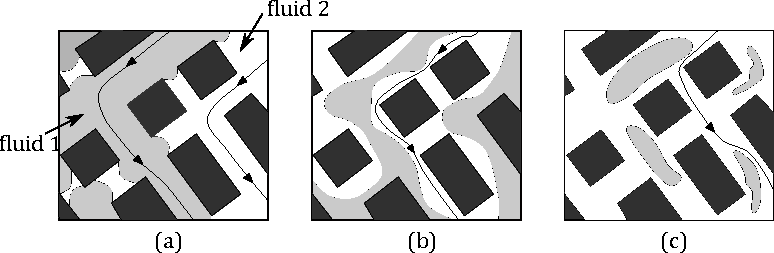
\includegraphics[scale=0.6]{figures/pdf/INTRODUCTION_fluidRepartitionSketch}
\par\end{centering}
\caption{Schematics of possible distributions of fluids in a 2D porous network
with solid phase in black, the non-wetting fluid (fluid 1) in light
grey, and the wetting fluid (fluid 2) in white, (a) the two fluids
are flowing in different channels separated by numerous meniscus and
the fluid-fluid interface extent is small, (b) the wetting and non-wetting
fluids are flowing together in most of the pores as two continuous
streams and (c) both fluids are flowing together in most of the pores
and the non-wetting phase is discontinuous. - Adapted from \citep{dullien2012porous}\label{fig:fluidPatterns}}
\end{figure}

Models used to describe two-phase flows in porous media are often
based on a direct extension of Darcy's equations for one-phase flow
\citep{wyckoff1936flow,muskat1938flow}. This generalization depends
on the introduction of relative permeabilities that essentially account
for the division of the available void space between the fluids; thus
each fluid phase acts as a supplementary solid regarding the other
one and no interaction between the phases is taken into account \citep{dullien2012porous,blunt2017multiphase}.
As a consequence, it is commonly assumed that the relative permeability
only depends on the saturation \citep{brooks1964hydrau,van1980closed}
and we know that this is not always accurate as relative permeabilities
may also depend on the capillary number \citep{Li2005}, the flow
regime \citep{Avraam1995} or the viscosity ratio \citep{yuster1951theoretical,ehrlich1993viscous,Yiotis2007}.
Since the early 1980s, numerous works have aimed at improving the
generalized Darcy equations on a sound physical basis. Using upscaling
techniques, several authors proposed additional coupling terms that
correspond to stresses at the fluid-fluid interface and yield coupling
permeability tensors \citep{MARLE1982643,auriault1986remarques,Whitaker1986a,Lasseux1996}.
The importance of these coupling terms in the overall flow process
is not clear \citep{ayub1999interfacial}. These additional terms
can be calculated analytically in a two-phase annular cocurrent flow
in a cylindrical capillary tube, and are of the same order as the
dominant relative permeabilities \citep{bacri1990modele}. However,
other studies considered configurations for which the surface between
fluids was smaller and concluded that coupling terms should not be
as important \citep{scott1953explanation,rakotomalala1995viscous}.
\citet{zarcone1994determination}, \citet{Dullien1996} and \citet{ramakrishnan2015measurement}\lyxadded{Maxime}{Fri Jun 26 12:11:51 2020}{
}directly measured the coupling permeability terms in natural media
by performing steady-state cocurrent two-phase flows. \citet{Rose1988}
proposed to indirectly measure the coupling relative permeability
terms by performing two different types of experiments. This technique
was also used for both cocurrent and countercurrent experiments \citep{bourbiaux1990experimental,bentsen1993use}.
Each of these authors, except Zarcone and Lenormand, found that the
coupling relative permeabilities are significant. Recently, \citet{clavier2017modeling}
performed experiments of inertial two-phase flows in coarse non-consolidated
porous media and proposed constitutive models. However, results suffer
from a major shortcoming. Indeed, it is impossible to know which type
of flow regime dominates at the pore scale and thus the exact link
between the physics at the pore-scale and the macroscale model.

Micromodels can be used to better understand two-phase flows in porous
media \citep{karadimitriou2012review}, e.g. transitions between the
flow regimes or the onset and development of displacement instabilities
\citep{lenormand1988numerical,zhang2011influence}. Therefore, micromodels
allow overcoming the major issue we have just risen. Such apparatus
were employed to measure the relative coupling permeabilites for different
flow regimes \citep{Avraam1995} or study the impact of the fluid-fluid
drag on the flow characteristics \citep{Heshmati2018,Roman2019}.
\citet{Rothman1990} used numerical simulations in a 2D micromodel
geometry and found that coupling permeabilities are comparable in
magnitude with the case of the annular flow in a capillary tube. Fig.~\ref{fig:comparison_Kr_litterature}
shows Rothman's results along with some of the previously mentioned
results on relative coupling permeabilities. Hele-Shaw cells are one
of the simplest example of micromodels as they consist of two parallel
plates in between which the fluids flow. Governing equations for the
flow in such cells are similar to Darcy's equation, and thus the permeability
can be easily modified by increasing or decreasing the aperture between
the plates \citep{saffman1958penetration}. Recently, this characteristic
has been used to investigate the flow paths of a two-phases flow as
a function of the micromodel thickness \citep{liu2019preferential}
or to study the stability of an immiscible two-phases displacements
in a Hele-Shaw cell with a spatially varying thickness \citep{jackson2017stability}.
Here, we study the influence of micromodel's absolute permeability
on the fluid-fluid drag and solid-fluids drag for different capillary
numbers. The original idea of the article is to solve the appropriate
depth-averaged equations for two-phase flows in a Hele-Shaw cell to
study the effect of the varying absolute permeability on the drag
forces without having to change the in-plane geometry.

\begin{figure}
\begin{centering}
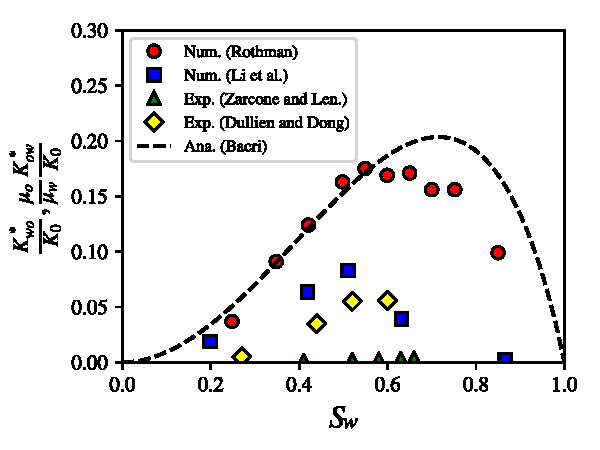
\includegraphics[scale=1.5]{figures/pdf/INTRODUCTION_littPerm}
\par\end{centering}
\caption{Normalized coupling relative permeabilities $K_{ij}^{*}$ as a function
of the wetting-fluid saturation $S_{w}$ from experimental work \citep{Dullien1996,zarcone1994determination},
numerical simulations \citep{Rothman1990,Li2005} and analytical solution
for a steady-state annular two-phase flow in a circular capillary
tube (dashed line) \citep{bacri1990modele}. The capillary theoretical
case provides an upper limit in terms of permeability and extent of
the interfacial surface area between the fluids. \label{fig:comparison_Kr_litterature}}

\end{figure}


\section{Pore-scale, depth-averaged and surface-averaged flow equations}

In this section, we present the derivation of the averaged flow equations
for two-phases flows in a Hele-Shaw cell, starting from the three-dimensional
Stokes equations. Then, we average the momentum equations spatially
to derive the unclosed form of the macroscopic momentum transport
equations. The system under consideration is depicted in Fig.~\ref{fig:Schematic_heleSahw}
which represents a quasi-planar cocurrent two-phase flow between two
parallel plates with a wedge of circular cross-section as a solid
obstacle. The transverse dimension of the cell is noted $L$ and $h$
is the length of the aperture between the plates.

\begin{figure}
\begin{centering}
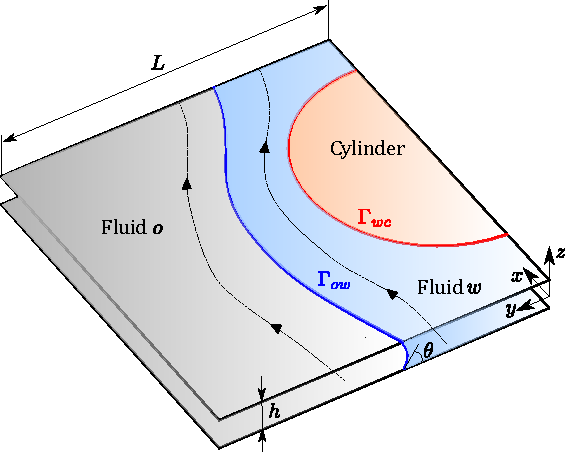
\includegraphics{figures/pdf/THEORY_heleShawSystemSketch}
\par\end{centering}
\caption{Schematic view of a cocurrent two-phase flow in a Hele-Shaw cell parallel
to the $x-y$ plane with a wedge of circular cross-section as a solid
obstacle. The transverse dimension of the cell is noted $L$ and $h$
stands for the aperture between the plates. The boundary between the
wetting-fluid $w$ and the cylinder (in red) is noted $\Gamma_{wc}$
and the boundary between the two fluids (in blue) is noted $\Gamma_{ow}$.
No dynamic films along the plates are considered here and $\theta$
stands for the non-zero contact angle between the two fluids and the
plates. \label{fig:Schematic_heleSahw}}
\end{figure}


\paragraph{Pore-scale flow equations}

Three-dimensional continuity and Stokes equations for a Newtonian
fluid in the absence of external forcing read, respectively,

\begin{equation}
\nabla^{*}\cdot\mathbf{u}=0,\qquad-\nabla^{*}p+\mu\nabla^{*2}\mathbf{u}=0,\label{eq:3dStokes}
\end{equation}

\noindent where the superscript {*} indicates that the derivative
operators are three-dimensional.

\paragraph{Depth-averaged flow equations}

\noindent The starting point is to consider an aparatus such as depicted
in Fig.~\ref{fig:Schematic_heleSahw} for which $h$ is very small
compared to the transverse length of the cell. It follows that the
$z$-component of the velocity can be neglected and

\begin{equation}
\mathbf{u}=\left(u(x,y,z),v(x,y,z),0\right)^{T}=f(z)\bar{\mathbf{u}}(x,y),
\end{equation}

\noindent where we introduce the depth-averaged velocity defined as
$\bar{\mathbf{u}}\equiv\frac{1}{h}\int_{-h/2}^{h/2}\mathbf{u}\:\mathrm{d}z$.
The in-plane version of Eq.~\ref{eq:3dStokes} then read

\begin{equation}
\nabla\cdot\bar{\mathbf{u}}=0,\qquad-\nabla p+\mu\left(\nabla^{2}\bar{\mathbf{u}}+\bar{\mathbf{u}}\frac{\partial^{2}f(z)}{\partial z^{2}}\right)=0.\label{eq:inPlaneStokes}
\end{equation}

\noindent From the condition $\int_{-h/2}^{h/2}f(z)\:\mathrm{d}z=h$,
arising from the definition of the depth-averaged velocity, along
with the no-slip boundary condition at $z\pm h/2$, we find that $f(z)=\frac{3}{2}(1-4\frac{z^{2}}{h^{2}})$.
Then,

\begin{equation}
\nabla\cdot\bar{\mathbf{u}}=0,\qquad\mu\left(\nabla^{2}\bar{\mathbf{u}}-k^{2}\bar{\mathbf{u}}\right)=\nabla p,\label{eq:amalgamStokesDarcy}
\end{equation}

\noindent are the continuity and momentum transport equations for
the depth-averaged flow of one fluid and $k=\sqrt{12}/h$. It has
been shown that the velocity profile for a flow in a rectangular channel
with Eq.~\ref{eq:amalgamStokesDarcy} lead to a reasonable approximation,
up to aspect ratios $h/L=1$, of the result obtained from the three-dimensional
Stokes equations \citep{nagel2015boundary}. In the case of two-phase
flows, these equations have to be written for each fluid and boundary
conditions at the fluid-fluid interfaces are required. Continuity
of the depth-averaged velocities across the interface and a jump of
interface normal stress are sufficient if the surface tension is constant
along the interface \citep{park1984two}. These conditions are expressed

\begin{equation}
\bar{\mathbf{u}}_{o}-\bar{\mathbf{u}}_{w}=0\;\textrm{at}\;\text{\ensuremath{\Gamma_{ow}}},
\end{equation}

\begin{equation}
\left(\bar{\boldsymbol{\sigma}}_{w}-\boldsymbol{\bar{\sigma}}_{o}\right)\cdot\mathbf{n}_{ow}=\gamma\left(\frac{\pi}{4}\kappa_{\parallel}+\frac{2}{h}\cos\theta\right)\mathbf{n}_{ow}\;\textrm{at}\;\text{\ensuremath{\Gamma_{ow}}},\label{eq:BCHeleShawStress}
\end{equation}

\noindent where $\bar{\boldsymbol{\sigma}}_{i}$ is the in-plane stress
tensor of fluid $i$, $\mathbf{n}_{ow}$ is the in-plane normal vector
at the fluid interface pointing toward the fluid $w$, $\gamma$ is
the surface tension, $\kappa_{\parallel}$ is the in-plane interface
curvature and $\theta$ denotes the contact angle between the fluid
interface and the plates (Fig.~\ref{fig:Schematic_heleSahw}). The
meniscus in the $z$-direction is approximated as a half-circle of
radius $h/2$ and the $\pi/4$ correction for the in-plane curvature
was derived by \citet{park1984two}. In Eq.~\ref{eq:BCHeleShawStress},
we neglected the additional terms that pertain to the formation of
the dynamic film \citep{park1984two} which scaled non-linearly with
the capillary number. We rather considered a non-zero contact angle,
and consequently, the absence of such thin films.

\paragraph{Volume-averaged flow equations}

Here, we proceed to the spatial averaging of the in-plane momentum
transport equations. We recall that all the flow variables and differential
operators have components only in the transverse direction. According
to the volume averaging framework \citep{Whitaker2013} and acknowledging
that Eq.~\ref{eq:amalgamStokesDarcy} are two-dimensional, the traditional
averaging theorem for the depth-averaged quantity $\bar{\omega}_{i}$
associated with the fluid $i$ reads

\begin{equation}
\langle\nabla\bar{\omega}_{i}\rangle=\nabla\langle\bar{\omega}_{i}\rangle+\frac{1}{S}\int_{\Gamma_{ic}}\mathbf{n}_{ic}\bar{\omega}_{i}\:\mathrm{d}\Gamma+\frac{1}{S}\int_{\Gamma_{ij}}\mathbf{n}_{ij}\bar{\omega}_{i}\:\mathrm{d}\Gamma,
\end{equation}

\noindent where,

\begin{equation}
\langle\bar{\omega}_{i}\rangle=\frac{1}{S}\int_{S_{i}}\bar{\omega}_{i}\:\mathrm{d}S,
\end{equation}

\noindent is the superficial surface average and $S$ is the surface
of a representative elementary cell. Applying the superficial surface
average of Eq.~\ref{eq:amalgamStokesDarcy} along with the averaging
theorem and using traditional length-scale arguments \citep{Whitaker2013}
we obtain

\begin{subequations}

\begin{equation}
\nabla\cdot\langle\bar{\mathbf{u}}_{i}\rangle=0,\quad i,j=o,w,\:i\neq j,
\end{equation}

\begin{multline}
\frac{1}{S}\int_{\Gamma_{ic}}\mathbf{n}_{ic}\cdot\left(-p_{i}\mathbf{I}+\mu_{i}\left(\nabla\bar{\mathbf{u}}_{i}+\left(\nabla\bar{\mathbf{u}}_{i}\right)^{T}\right)\right)\:\mathrm{d}\Gamma+\\
+\frac{1}{S}\int_{\Gamma_{ij}}\mathbf{n}_{ij}\cdot\left(-p_{i}\mathbf{I}+\mu_{i}\left(\nabla\bar{\mathbf{u}}_{i}+\left(\nabla\bar{\mathbf{u}}_{i}\right)^{T}\right)\right)\:\mathrm{d}\Gamma-\\
-\mu_{i}k^{2}\langle\bar{\mathbf{u}}_{i}\rangle=\varepsilon_{i}\nabla\langle p_{i}\rangle^{i}+\langle p_{i}\rangle^{i}\nabla\varepsilon_{i},\quad i,j=o,w,\:i\neq j,\label{eq:averagedFull}
\end{multline}

\end{subequations}

\noindent where $\mathbf{I}$ is the $2\times2$ identity matrix and
$\langle p_{i}\rangle^{i}$ $\left(\langle p_{i}\rangle^{i}=\langle p_{i}\rangle/\varepsilon_{i}\right)$
is the intrinsic surface average pressure of fluid $i$, with $\varepsilon_{i}$
the volume fraction of fluid $i$. The first integral is the drag
force exerted upon the cylinders boundary by fluid $i$ and the second
integral pertains for the drag force exerted upon fluid $j$ by fluid
$i$. Here, we consider that the contour of the fluid-fluid interface
in the $x-y$ plane can be identically translated along the $z$-direction,
which is an approximation since the meniscus is a half-circle for
small $h/L$ ratio. However, as shown in the Appendix~\ref{sec:Approximation-made},
using three-dimensional flow simulations in microchannels, these approximations
remain reasonable.

If the variation of the saturation in space is negligible and acknowledging
that, as illustrated in Fig.~\ref{fig:Schematic_heleSahw}, only
the wetting fluid $w$ is in contact with the wedge, a more compact
form of Eq.~\ref{eq:averagedFull} reads

\vspace{-12mm}

\begin{subequations}

\begin{alignat}{1}
0 & =-\varepsilon_{w}\nabla\langle p_{w}\rangle^{w}-\mu_{w}k^{2}\langle\bar{\mathbf{u}}_{w}\rangle+\mathbf{d}_{wc}+\mathbf{d}_{wo},\\
0 & =-\varepsilon_{o}\nabla\langle p_{o}\rangle^{o}-\mu_{o}k^{2}\langle\bar{\mathbf{u}}_{o}\rangle+\mathbf{d}_{ow},
\end{alignat}

\end{subequations}

\noindent Here, $\mathbf{d}_{ij}$ ($\mathbf{d}_{ij}=\int_{\Gamma_{ij}}\boldsymbol{\sigma}_{i}\cdot\mathbf{n}_{ij}\:\mathrm{d}\Gamma$)
denotes the drag forces per unit surface area exerted upon phase $j$
by phase $i$ and which must be computed or modeled to obtain closed
macroscopic equations. In the following, we are working on the direct
calculation of each drag force terms summarized in Tab.~\ref{tab:Summary-of-each-drag}.

\begin{table}
\begin{centering}
\begin{tabular}{cccc}
\toprule 
\begin{tabular}{c}
Drag of\tabularnewline
upon\tabularnewline
\end{tabular} & Fluid $o$ & Fluid $w$ & \tabularnewline
\midrule
\midrule 
Plates & $-\mu_{o}\langle\bar{\mathbf{u}}_{o}\rangle\frac{12}{h^{2}}$ & $-\mu_{w}\langle\bar{\mathbf{u}}_{w}\rangle\frac{12}{h^{2}}$ & \multirow{2}{*}{$\Sigma=\mathbf{d}_{s}$}\tabularnewline
\cmidrule{1-3} \cmidrule{2-3} \cmidrule{3-3} 
Wedge & - & $\mathbf{d}_{wc}$ & \tabularnewline
\midrule 
Fluid $o$ & - & $\mathbf{d}_{wo}$ & \multirow{2}{*}{$\Sigma=\mathbf{d}_{f}$}\tabularnewline
\cmidrule{1-3} \cmidrule{2-3} \cmidrule{3-3} 
Fluid $w$ & $\mathbf{d}_{ow}$ & - & \tabularnewline
\bottomrule
\end{tabular}
\par\end{centering}
\caption{Summary of each drag force terms involved in the averaged momentum
transport equation for two-phase flow in a Hele-Shaw cell.\label{tab:Summary-of-each-drag}}
\end{table}


\section{Direct numerical simulations}

In this section, we introduce the standard Level Set method to capture
the moving free interface between the fluids, along with the flow
equations, both solved with a Finite Element solver.

\subsection{Equations}

\paragraph{Level Set model}

The Level Set method is an Eulerian method that easily handles the
topological phases changes, in contrast with Lagrangian methods. Here,
the fluid phases are identified with a phase color function that goes
smoothly from 0 to 1 across the fluid interface with the manifold
defined as the iso-level $\phi=0.5$. Transport of the level set function
$\phi$ is governed by

\begin{equation}
\frac{\partial\phi}{\partial t}+\nabla\cdot(\bar{\mathbf{u}}\phi)=\tau\nabla\cdot\left(\psi\boldsymbol{\nabla}\phi-\phi(1-\phi)\frac{\boldsymbol{\nabla}\phi}{\vert\nabla\phi\vert}\right),\label{eq:advecPhi}
\end{equation}

\noindent where $\bar{\mathbf{u}}$ is the depth-averaged velocity
field and $\tau$ and $\psi$ are two numerical parameters that control
the diffuse interface thickness and the amount of initialization of
$\phi$ function, respectively \citep{Olsson2007}. We investigated
the accuracy of the implicit definition of the interface as well as
the effect of the value of the initialization parameter on the interface
position in Appendix~\ref{sec:Comparison-with-BEM} by comparing
to a boundary element method \citet{nagel2015boundary}.

The governing flow equations read

\vspace{-12mm}

\begin{subequations}

\begin{alignat}{1}
0 & =\nabla\cdot\bar{\mathbf{u}}\\
0 & =-\nabla p+\mu(\phi)\left(\nabla^{2}\bar{\mathbf{u}}-\frac{12}{h^{2}}\bar{\mathbf{u}}\right)+\gamma\left(\frac{\pi}{4}\nabla\cdot\left(\frac{\boldsymbol{\nabla}\phi}{\vert\boldsymbol{\nabla}\phi\vert}\right)-\frac{2}{h}\right)\delta(\phi)\mathbf{n},\label{eq:Momentum-1}
\end{alignat}

\end{subequations}

\noindent where $\delta$ is the Dirac delta function localized on
the interface and $\mathbf{n}$ denotes the unit normal to the interface,
respectively defined as,

\begin{equation}
\delta(\phi)=6\left|\boldsymbol{\nabla}\phi\right|\left|\phi\left(1+\phi\right)\right|,\quad\textrm{and}\quad\mathbf{n}=\frac{\boldsymbol{\nabla}\phi}{\left|\boldsymbol{\nabla}\phi\right|}.
\end{equation}

\noindent We introduce the following reference and dimensionless quantities,

\begin{equation}
\bar{\mathbf{u}}=\bar{\mathbf{u}}'\times U_{r},\;p=p'\times\frac{\mu_{r}U_{r}}{L},\;\mathbf{x}=\mathbf{x}'\times L,\label{eq:referenceQuantities}
\end{equation}

\noindent and the dimensionless continuity and momentum transport
equations are

\vspace{-12mm}

\begin{subequations}

\begin{alignat}{1}
0 & =\nabla'\cdot\bar{\mathbf{u}}'\\
0 & =-\nabla'p'+\frac{\mu(\phi)}{\mu_{r}}\left(\nabla'^{2}\bar{\mathbf{u}}'-\frac{12}{\left(h/L\right)^{2}}\bar{\mathbf{u}}'\right)+\frac{\gamma}{\mu_{r}U_{r}}\left(\frac{\pi}{4}\nabla'\cdot\left(\frac{\boldsymbol{\nabla'}\phi}{\vert\boldsymbol{\nabla'}\phi\vert}\right)-\frac{2}{h/L}\right)\delta'(\phi)\mathbf{n},\label{eq:dimensionlessMomentum}
\end{alignat}

\end{subequations}

\noindent with $\delta'(\phi)=6\left|\boldsymbol{\nabla'}\phi\right|\left|\phi\left(1+\phi\right)\right|$.
We therefore have three dimensionless numbers: the viscosity ratio
$M(\phi)=\frac{\mu(\phi)}{\mu_{r}}$, the capillary number $Ca^{-1}=\frac{\gamma}{\mu_{r}U_{r}}$
and the aspect ratio $h^{*}=h/L$.

\paragraph{Geometry, boundary conditions and simulation parameters}

Our macroscopic model is a Hele-Shaw cell with wedges of cylindrical
cross-section. This system is subdivided into seven unit-cell (UC)
subdomains encompassing one wedge, as depicted in Fig.~\ref{fig:model}.
Taking advantage of the symmetry, we studied only the upper half of
a row. Each fluid flows from left to right ($x$-direction) and the
inlet boundary conditions for both fluids are a constant normal inlet
velocity $u_{i}$. The outlet boundary condition for the flow is a
reference pressure. The boundary conditions used are summarized in
Tab.\ref{tab:Boundary-conditions}. We choose the total inlet velocity
as the reference velocity; thus the dimensionless inlet velocities
can be expressed as a fractional flow $f_{f}$,

\begin{equation}
f_{f}=\frac{u_{w}}{U_{t}},\quad u_{o}=1-f_{f},\quad\textrm{with}\quad U_{t}=u_{w}+u_{o}.
\end{equation}

\noindent The non-wetting viscosity is taken as the reference viscosity
and the respective value of each dimensionless parameters is in Tab.~\ref{tab:Boundary-conditions}.
The initialization parameter value is equal to the maximum inlet velocity
value, which yields maximum accuracy (Appendix~\ref{sec:Comparison-with-BEM}).
As a reference, we conducted numerical simulations of one-phase flows
and found that the range of aperture corresponds to a range absolute
permeabilities between $1.5\times10^{4}$ and $40$ darcy. 
\begin{figure}
\begin{centering}
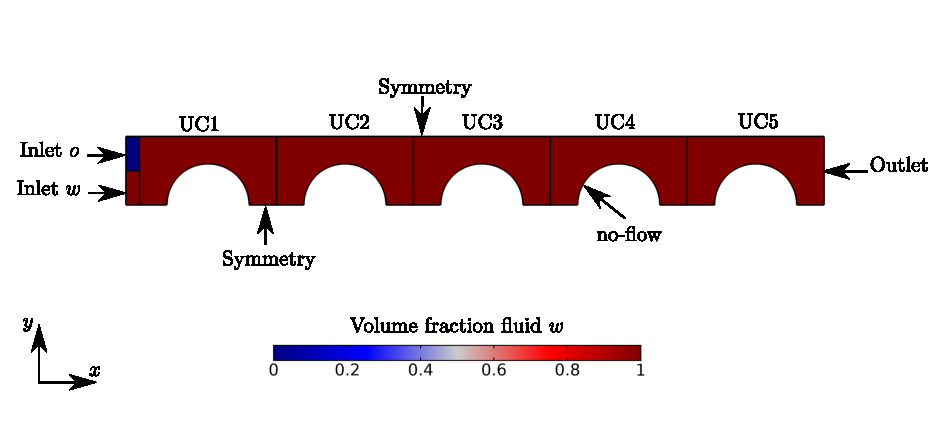
\includegraphics{figures/pdf/DNS_model}
\par\end{centering}
\caption{Schematics of the geometry and initial condition. We consider the
superior half of an array of five cylindrical wedges inside five cuboids
where both fluids are injected from left to right. Initially, the
model is saturated with wetting fluid (red), and the width $L$ of
one Unit Cell (UC) is $5\times10^{-4}$ m. Symmetry boundary conditions
are used on both length sides and the no-flow boundary condition is
imposed at the wedge boundary. \label{fig:model}}
\end{figure}

\begin{table}
\caption{Boundary conditions for flow variables and the Level Set function
(left) and simulation parameters (right).\label{tab:Boundary-conditions}}

\centering{}%
\begin{tabular}{cccc}
\toprule 
Boundary & $u$ & $p$ & $\ensuremath{\phi}$\tabularnewline
\midrule
\midrule 
Outlet & - & $0$ & $\mathbf{n}\cdot\boldsymbol{\nabla}\phi=0$\tabularnewline
\midrule 
Inlet $o$ & $u_{o}$ & - & $0$\tabularnewline
\midrule 
Inlet $w$ & $u_{w}$ & - & $1$\tabularnewline
\bottomrule
\end{tabular}\hfill{}%
\begin{tabular}{cc}
\toprule 
Parameters & Value\tabularnewline
\midrule
\midrule 
$Ca=\frac{U_{t}\mu_{o}}{\gamma}$ & from $0.5$ to $0.02$\tabularnewline
\midrule 
$M_{w}=\frac{\mu_{w}}{\mu_{o}}$ & 1\tabularnewline
\midrule 
$f_{f}=\frac{u_{w}}{U_{t}}$ & 1/4\tabularnewline
\midrule 
$h^{*}=h/L$ & from $5$ to $1/20$\tabularnewline
\bottomrule
\end{tabular}
\end{table}


\paragraph{Mesh convergence study}

Here, we study the mesh convergence of the various drag forces. The
dimensionless numbers for this study are $Ca=0.5$, $h^{*}=1/4$,
$f_{f}=0.25$ and $M=1$. In Fig.~\ref{fig:Mesh-convergence-study}
(a) the results are normalized with respect to the finer mesh result
and are given as a function of the total number of degree of freedom
in the whole model. The fluid-fluid interface position for three different
mesh densities is given in Fig.~\ref{fig:Mesh-convergence-study}
(b). We obtain these results in the fourth unit-cell (UC4) at steady-state.
The drag terms are not very sensitive to the mesh density and the
interface between the fluids is correct even for a coarse mesh and
converges quickly. In the following simulations, we use a mesh that
corresponds to $3.7\times10{{}^5}$ degree of freedoms

\begin{figure}[H]
\begin{centering}
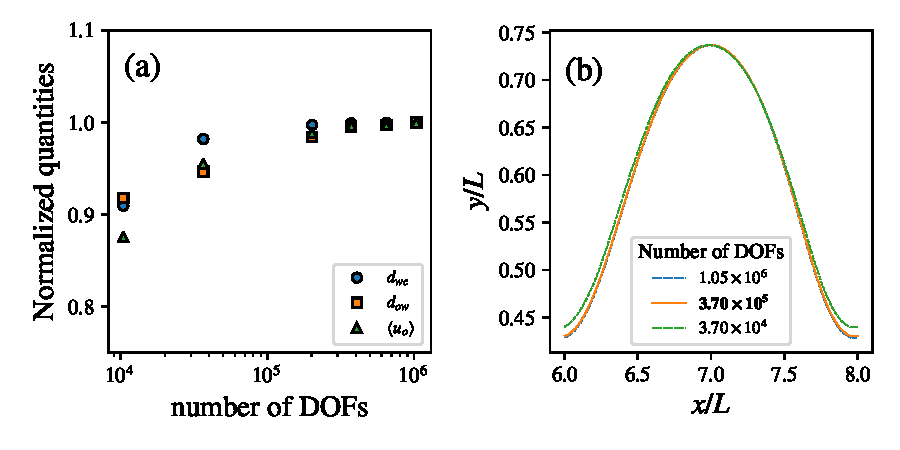
\includegraphics{figures/pdf/DNS_meshConv}
\par\end{centering}
\caption{Mesh convergence study of (a) drag force exerted upon the wedge (red),
drag force exerted upon the fluid-fluid boundary (blue) and intrinsic
average velocity of fluid $o$ (green) . All the results are normalized
with respect to the result obtained with the finer mesh, at steady-state
and in UC4. (b) Fluid-fluid interface position in UC4 at steady-state
for different number of degree of freedoms in the whole geometry.
Flow parameters are $Ca=0.5$, $h^{*}=1/4$, $f_{f}=0.25$ and $M=1$.
In the following we use a mesh that corresponds to $3.7\times10{{}^5}$
degree of freedoms.\label{fig:Mesh-convergence-study}}
\end{figure}


\section{Results and discussion}

Before presenting the results for drag force terms, we briefly discuss
the two-phase flow regime observed along with the variation of the
saturation with time. The flow regime is fundamental as it drives
the extent of the interfacial surface area between the fluids.

\paragraph{Two-phase flow regimes}

We observe that the two fluids remain continuous at all times and
for the entire range of tested capillary numbers and aperture. The
interface between the fluids becomes stationary and a stationary state
is reached for every capillary number and aperture values. Fig.~\ref{fig:Fluid-repartion-along}
shows the initial, intermediate, and final configurations of the fluid
repartition for the case $Ca=1\times10^{-1}$ and $h^{*}=1/8.$ At
steady-state, the fluid-fluid interface is periodic on the five central
unit cells whereas the interface is slightly deformed at the inlet
and outlet cells, under the influence of boundary conditions.

We could have expected a break-up of the invading phase either by
snap off phenomena, or by the shear action of the wetting fluid flow.
However, the pore throat is large and the fractional flow is low,
which favours the continuity of the fluid phases. The flow regime
observed is therefore a film-flow regime within the limit of the parameters
chosen for this study. We obtained all the following results in the
fourth unit-cell (UC4) in order to be far from the influence of the
inlet and outlet boundary conditions.

\begin{figure}
\begin{centering}
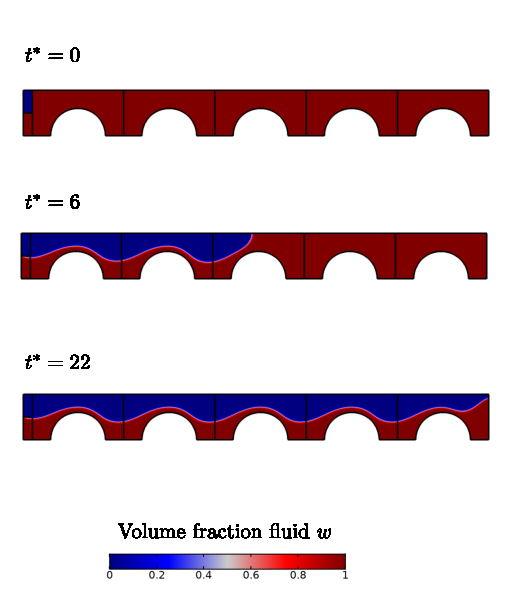
\includegraphics[scale=1.2]{figures/pdf/RESULTS_dynamic}
\par\end{centering}
\caption{Fluids repartion along the superior half-row at (a) the initial time,
(b) for an intermediate time and (c) final time (steady-state reached)
for $Ca=0.1$, $f_{f}=0.25$, $M=1$ and $h^{*}=1/8$. At steady-state
the fluid-fluid interface taken on the central unit cells is periodic
whereas it is slightly deformed in the first and last UC under the
influence of the boundary conditions. \label{fig:Fluid-repartion-along}}
\end{figure}


\paragraph{Saturation}

Wetting fluid saturation at steady-state decreases, in average, from
0.6 to 0.4 as the aperture between the plates decreases from 5 to
1/20. This can be seen in Fig.~\ref{fig:wettingFluidSaturation},
which presents the saturation in UC4 as a function of the dimensionless
aperture and for different capillary numbers. The saturation does
not depend on the capillary number for the smallest apertures. However,
as the aperture between the plates increases, the fluid-fluid interface
becomes flatter and the saturation of the wetting fluid increases
until it converges to the saturation obtained for the 2D limit case
which values slightly depend on the capillary number (see saturation
fields insets in Fig.~\ref{fig:wettingFluidSaturation}). Fig.~\ref{fig:Comparison-of-interface}
compares the position of the fluid-fluid interface in UC4 for different
aperture and capillary numbers. For $Ca=5\times10^{-1}$ the interface
is symmetric regardless the aperture's value, whereas the interface
is non-symmetric for low $Ca$ and small aperture.

\begin{figure}
\begin{centering}
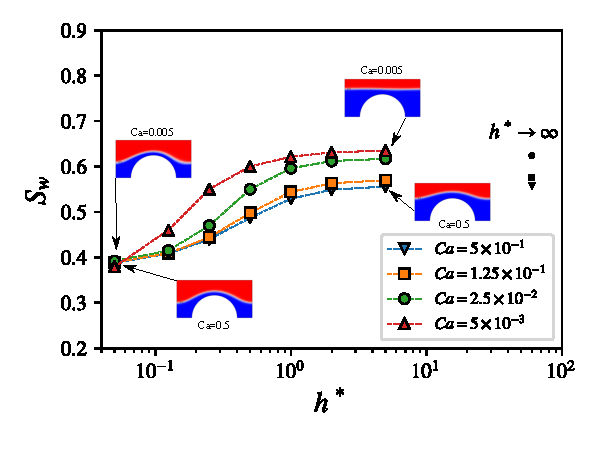
\includegraphics[scale=1.5]{figures/pdf/RESULTS_saturation}
\par\end{centering}
\caption{Fluid saturation at steady-state in UC4 as a function of the dimensionless
aperture and for different capillary numbers. Fields of the level-set
function at steady-state in UC4 are given for the selected value of
the dimensionless aperture and $Ca=5\times10^{-1}$ and $Ca=2\times10^{-2}$.
As the aperture increases the interface flattens and the wetting fluid
saturation increases. A decrease in the capillary number acts in the
same way, albeit less strongly. The 2D limit case is given with plain
black markers. \label{fig:wettingFluidSaturation}}
\end{figure}

\begin{figure}
\begin{centering}
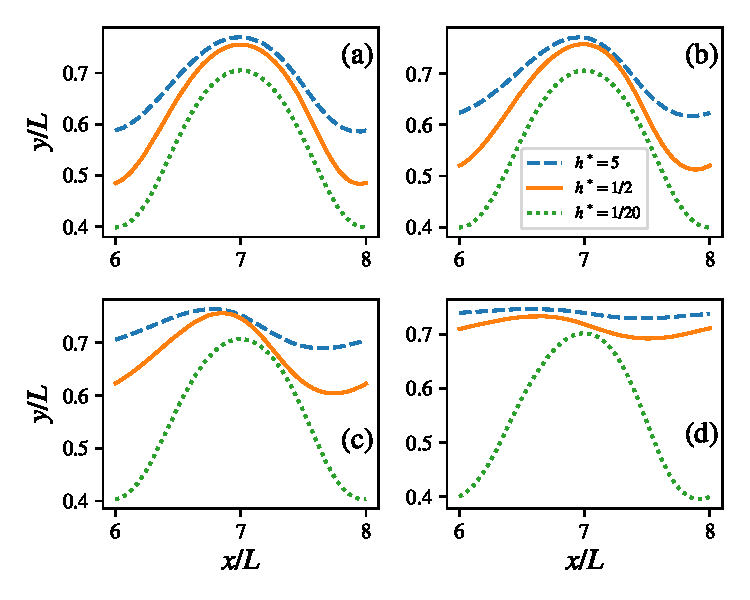
\includegraphics{figures/pdf/RESULTS_interfacePosition}
\par\end{centering}
\caption{Comparison of interface position for different aperture (a) $Ca=5\times10^{-1}$and
(b) $Ca=2\times10^{-2}$ (in UC4 for $f_{f}=0.25$ and $M=1$).\label{fig:Comparison-of-interface}}
\end{figure}


\paragraph{Drag force}

We compute the fluid-fluid drag according to Eq.\ref{eq:averagedFull}.
The viscous part is obtained through the velocity gradient available
at the $\phi=0.5$-contour and the pressure part is obtained by application
of the divergence theorem. In the following, we are interested in
the drag force component in the $x$-direction, i.e., the main flow
direction. The drag force exerted upon the solid-fluids boundaries,
denoted $d_{s}^{x}$, is the sum of the drag upon the wedge and upon
the cell plates by both fluids, as defined in Tab~\ref{tab:Summary-of-each-drag}.
The fluid-fluid drag, denoted $d_{f}^{x}$, is the sum $d_{f}^{x}=d_{ow}^{x}+d_{wo}^{x}$.
In the following, the $x$–component of the drag forces are expressed
per unit surface area of unit-cell.

Fig.~\ref{fig:ratioDragForceTotal} shows the ratio of the fluid-fluid
drag over the solid-fluid drag as a function of the aperture between
the plates and different values of capillary number. \lyxadded{Maxime}{Wed Jul  1 11:01:27 2020}{Our
results show that the fluid-fluid drag is non-negligible compared
to the solid-fluid drag. At most, the fluid-fluid drag reaches 80\%
of the value of the solid-fluid drag and this occur for high $Ca$
and large aperture. The results from the purely 2d simulations ($h^{*}\rightarrow\infty)$
indicate that for $h/L=5$, the larger aperture tested, the contribution
of the drag upon the plates is already insignificant. Then, by narrowing
the aperture, the fluid-fluid drag decreases compared to the solid-fluid
drag, until $h^{*}=1/2$. From $h^{*}=1/2$ and below the fluid-fluid
drag either remains constant, for the higher Ca, or increases. In
the end, for the smallest aperture, the importance of the fluid-fluid
drag does not depend on the capillary number and is 40\% of the value
of the solid-fluid drag.}

\lyxadded{Maxime}{Wed Jul  1 11:02:24 2020}{Regarding the limit case
of infinite aperture the capillary number is important}

\begin{figure}
\begin{centering}
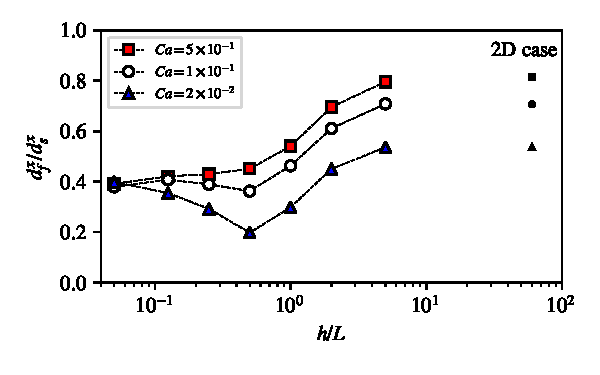
\includegraphics[scale=1.5]{figures/pdf/RESULTS_ratioDrag}
\par\end{centering}
\caption{Ratio of fluid-fluid drag force over solid-fluid drag force as a function
of the dimensionless aperture and for different capillary numbers
(in UC4 for $f_{f}=0.25$ and $M=1$). The 2D limit case is given
with plain black markers. \label{fig:ratioDragForceTotal}}
\end{figure}

Fig.~\ref{fig:Fluid-fluid-and-solid-fluid} shows the fluid-fluid
ant the solid-fluid drag forces as a function of the aperture and
for two capillary numbers. Here again, the dimensionless aperture
$h^{*}=1/2$ signal a change in the drag behavior. For $1/2<h^{*}$,
the fluid-fluid and solid-fluid drag forces barely change with the
aperture whereas, for $h^{*}<1/2$ both drag forces scale approximately
as $h^{-2}.$

\begin{figure}
\begin{centering}
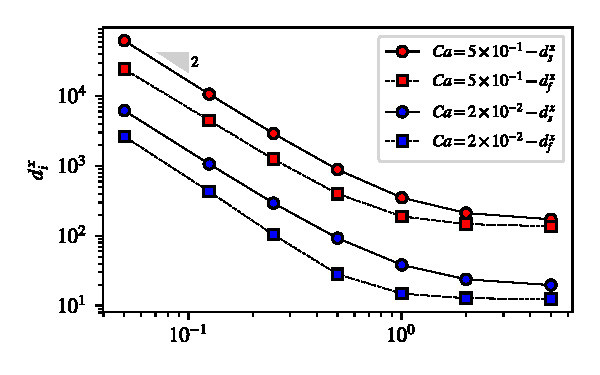
\includegraphics[scale=1.5]{figures/pdf/RESULTS_Drag}
\par\end{centering}
\caption{Comparison of fluid-fluid and solid-fluid drag force as a function
of the dimensionless aperture for two capillary numbers (in UC4 for
$f_{f}=0.25$ and $M=1$).\label{fig:Fluid-fluid-and-solid-fluid}}
\end{figure}

Fig.~\ref{fig:Proportion-solid--drag} shows the proportion of the
solid-fluid drag which is due to the drag exerted upon the wedge as
a function of the aperture. Here the 2D limit case is clear since
the solid-fluid drag is only due to the drag upon the wedge in that
case. The importance of the drag upon the wedge decreases as the aperture
decrease, however it remains non-negligible (40\% of the solid-fluid
drag) even for the smallest aperture $h^{*}=1/20$.

\begin{figure}
\begin{centering}
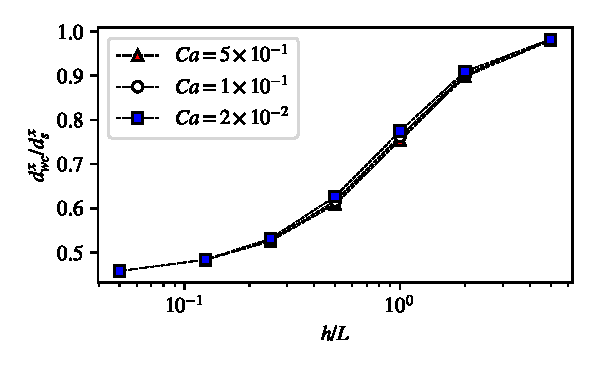
\includegraphics[scale=1.5]{figures/pdf/RESULTS_solidDrag}
\par\end{centering}
\caption{Proportion of the solid-fluid drag force due to the contribution of
the drag exerted upon the wedge, as a function of the dimensionless
aperture and for different capillary numbers (in UC4 for $f_{f}=0.25$
and $M=1$). \label{fig:Proportion-solid--drag}}
\end{figure}

Fig.~\ref{fig:Proportion-of-pressureTerm} shows the proportion of
the fluid-fluid and solid-fluid drag upon the wedge which is due to
the pressure part of the stress-tensor. The pressure part produces
most of the drag force, either regarding the fluid-fluid or the solid-fluid
drag upon the wedge, for $h^{*}<1/2$. For larger aperture, the fluid-fluid
drag is mainly produced by the viscous part, whereas the pressure
part has a minimum contribution as high as 60\% of $d_{wc}$.

\begin{figure}
\begin{centering}
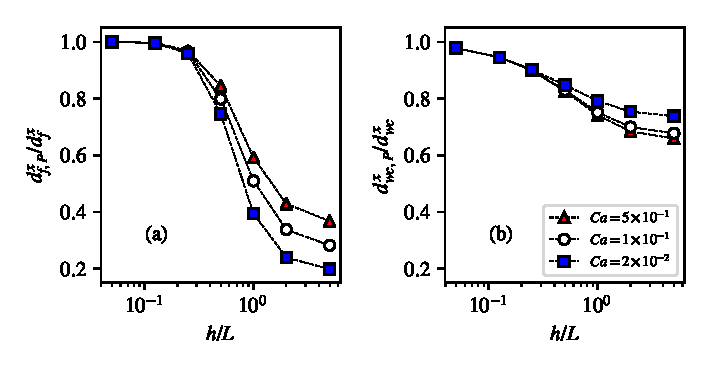
\includegraphics[scale=1.3]{figures/pdf/RESULTS_decompose}
\par\end{centering}
\caption{Proportion of the fluid/fluid drag (a) or the solid-fluid drag upon
the wedge (b) due to the pressure term contribution, as a function
of the dimensionless aperture and for different capillary numbers
(in UC4 for $f_{f}=0.25$ and $M=1$) \label{fig:Proportion-of-pressureTerm}}
\end{figure}

\begin{figure}
\begin{centering}
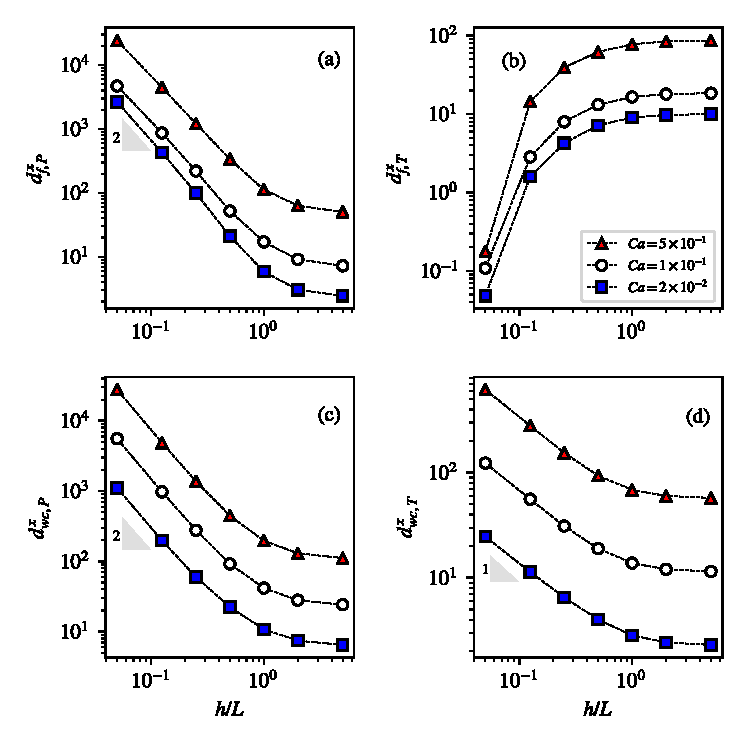
\includegraphics{figures/pdf/RESULTS_details}
\par\end{centering}
\caption{Comparison of the drag produced by the pressure for}
\end{figure}


\section{Conclusion}

In this study we conducted direct simulations of depth-averaged two-phases
flows, and we investigated the effect of the permeability on the drag
forces exerted upon the different phase interfaces. The permeability
was changed by varying the Darcean term which arising from the depth-averaging,
thus without altering the in-plane geometry. These drag terms have
to be modelled to obtain the macroscopic momentum transport equations
but the drag exerted upon the the fluid-fluid interface is commonly
neglected for flow driven by capillarity forces. Here we focused on
film-flow regime pourencountered in two-phases flows in high permeability
porous media or in microfluidic devices. We found that the drag exerted
upon the fluid-fluid interface should not be neglected into the momentum
transport equations for film-flow regimes. Lower permeability does
not make the drag force terms at the interface negligible as long
as the flow regime remains a film regime. On the contrary, the fluid-fluid
drag force increases faster than the drag upon the fluid-solid interfaces,
as the aperture between the plates decreases.  

\newpage{}

\bibliographystyle{elsarticle-harv}
\bibliography{biblio}

\newpage{}

\appendix

\section{Approximation made on the drag force when considering a fluid-fluid
flat interface\label{sec:Approximation-made}}

We conduct three-dimensional one-phase flow simulations into a microchannel
to determine the approximation made on the drag calculation when considering
that the fluid-fluid contour can be translated along the $z$-direction.

One side of the microchannel is a half-circle wall to mimic a fluid-fluid
interface whereas the opposite side is a flat wall (Fig.~\ref{fig:Microchannel}).
We obtain the curved side by extruding a cylinder; thus a special
treatment is done to correctly meshed the very thin part left, and
we build very small chamfers (Fig.~\ref{fig:Microchannel}). We compute
the drag force per unit surface area on each sidewall of the microchannel
and plot in Fig.~\ref{fig:Drag-force-exerted} the drag force exerted
upon the curved side normalized with respect to the flat wall. The
drag per unit surface area exerted upon the curved wall is roughly
70\% of the drag per unit surface area upon the flat wall. Giving
the greater extent of surface area for the curved wall, the difference
regarding the drag value is negligible.

\begin{figure}
\begin{centering}
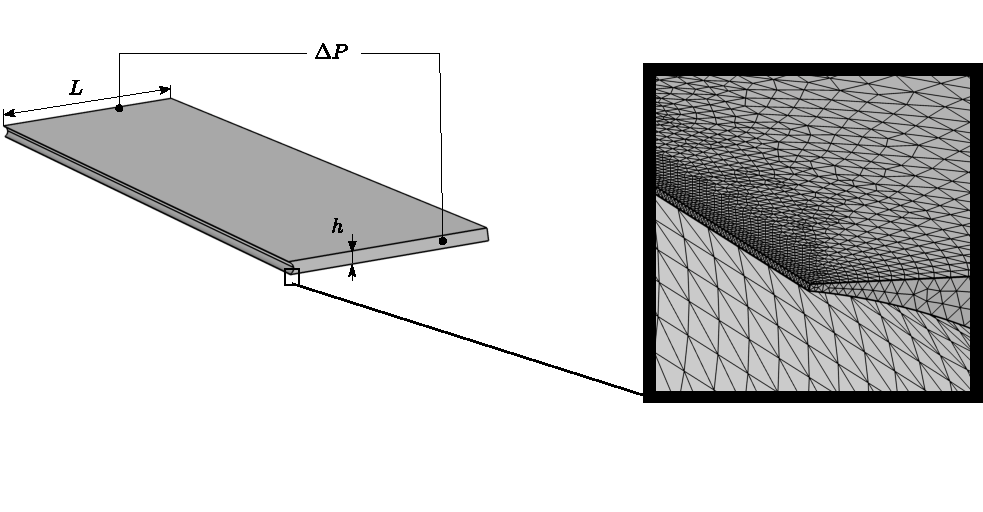
\includegraphics[scale=0.7]{figures/pdf/APPENDIX_microchannel}
\par\end{centering}
\caption{Microchannel with one side is a half-circle wall and the opposite
side is a flat wall with $h/L=1/16$ (left) and mesh detail at the
small chamfer build after the cylinder extrusion (right).\label{fig:Microchannel}}
\end{figure}

\begin{figure}
\begin{centering}
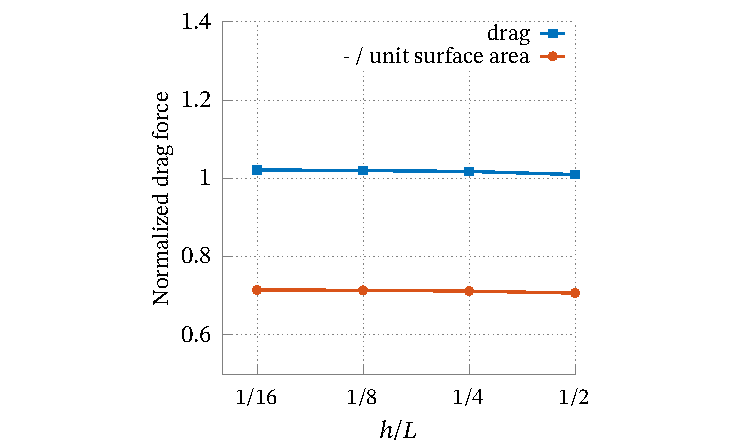
\includegraphics[scale=0.7]{figures/pdf/APPENDIX_test_half_circle}
\par\end{centering}
\caption{Drag force and drag force per unit surface area exerted upon the curved
wall of the microchannel normalized with respect to the drag force
exerted upon the flat wall. The drag exerted upon the curved solid
wall is almost equal to the drag exerted upon the flat wall, since
the smaller drag per unite surface area is almost fully compensated
by the greater surface area. \label{fig:Drag-force-exerted}.}
\end{figure}


\section{Comparison with a Boundary Element Method\label{sec:Comparison-with-BEM}}

Here we validate the Level Set (LS) code by comparison with a Boundary-Element
Method (BEM) \citep{nagel2015boundary}, which relies on a surface
discretization of the interface and a pseudo-analytical formulation
in the bulk of the phases. This allows us to precisely locate the
interface, even in the case of very thin film flow, and to carefully
analyze the choice of parameters in Eq.~\ref{eq:advecPhi}.

The test case resembles the case study (Fig.~\ref{fig:Test-case}).
The model is initially fully saturated with fluid $w$, with the exception
of the channel through which fluid $o$ is injected. We test either
the $\phi=0.5$ contour is an appropriate definition for the fluid-fluid
interface and in what extent the value of the initialization parameter
$\psi$ can change the interface position. In Fig.~\ref{fig:Interface-position}
we present the half-part of the model and the interface between the
fluids at time $t=2.5$, for an aspect ratio $h/L$, where $L$ is
the width of the fluid $o$ inlet channel. We present three different
interfaces obtained with the LS method, depending on the initialization
parameter value. This parameter is normalized with respect to the
inlet velocity of fluid $o$, which is three times greater than the
fluid $w$ inlet velocity. One can clearly observe that the interface
position obtained with the LS method is almost identical to that obtained
with the BEM, regardless of value of $\psi$. However, the best results,
especially regarding the interface tip position, is obtained for $\psi=U_{o}^{\mathrm{inlet}}$.

\begin{figure}
\begin{centering}
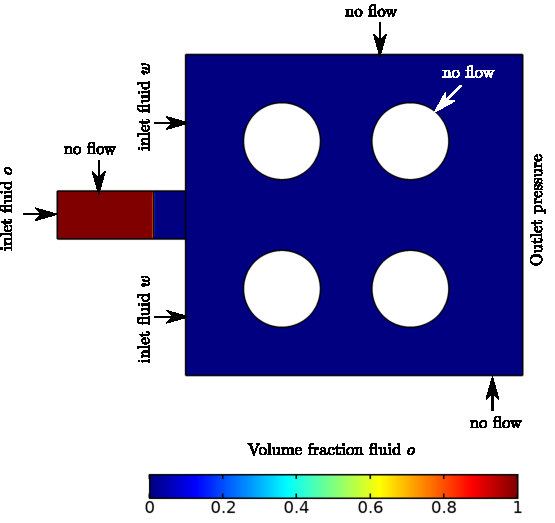
\includegraphics{figures/pdf/APPENDIX_compare_model_BEM}
\par\end{centering}
\caption{Test case for comparison between Level Set and Boundary Element methods.
The flow is cocurrent from left to right and the viscosity is the
same for both fluids.\label{fig:Test-case}}

\end{figure}

\begin{figure}
\begin{centering}
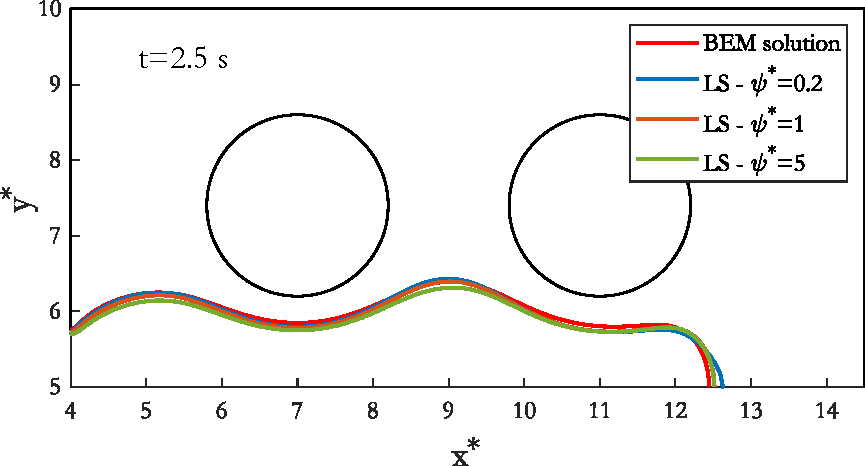
\includegraphics[scale=0.75]{figures/pdf/APPENDIX_interface_BEMvsLS}
\par\end{centering}
\caption{Interface position at time $t=2.5\:\mathrm{s}$ obtained for an aspect
ratio $h/L=0.25$ with a Boundary Element method and the Level Set
method for different values of the dimensionless initialization parameter
$\psi^{*}=\psi/U_{o}^{\mathrm{inlet}}$. \label{fig:Interface-position}}

\end{figure}

\end{document}
